%!TEX encoding = UTF-8 Unicode
% -*- coding: UTF-8; -*-
% vim: set fenc-utf-8

\chapter{Cas d'utilisations}
\label{s:cas_utilisation}

Ce chapitre présente les différents cas d'utilisation pour l'application VisuaLigue.
La figure \ref{fig:cas_utilisation_diag} résume les acteurs du systèmes et les cas d'utilisations.
La suite du chapitre décrit en détails les cas d'utilisations et s'attarde sur les plus importants.

\begin{figure}[htpb]
    \centering
    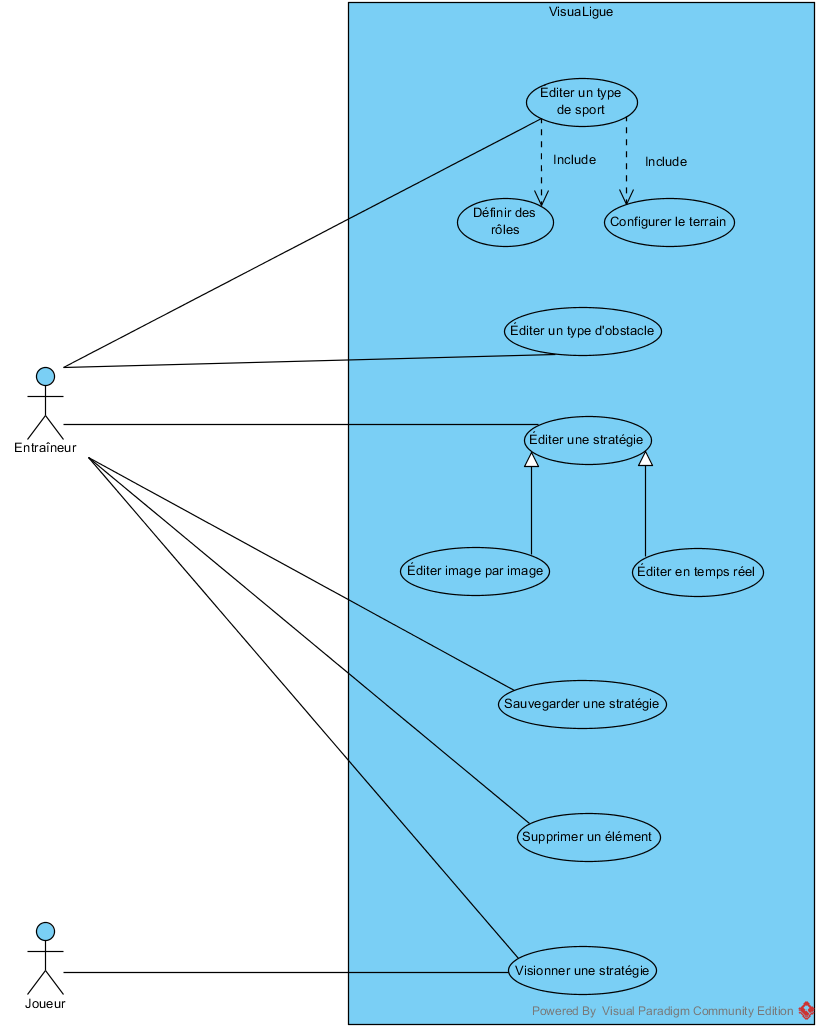
\includegraphics[scale=0.7]{fig/cas_utilisation_diag.png}
    \caption{Diagramme des cas d'utilisations}
    \label{fig:cas_utilisation_diag}
\end{figure}

\newpage



\section{Éditer un type de sport}
\label{sec:ajouter_un_type_de_sport}

\begin{itemize}
    \item \textbf{Cas d'utilisation:} Éditer un type de sport
    \item \textbf{Syst\`eme:} VisuaLigue
    \item \textbf{Acteur principal:} Entra\^ineur
    \item \textbf{Pr\'erequis:} Aucun.
    \item \textbf{Parties prenantes et int\'er\^ets:}
    	\begin{itemize}
    		\item Entraîneur : Veut pouvoir cr\'eer facilement le type de sport que pratique son équipe ainsi que configurer les paramètres de ce sport. 
    	\end{itemize}
    \item \textbf{Garanties en cas de succ\`es :} Le sport est ajout\'e \`a la liste des sports existants et peut \^etre utiliser lors de la cr\'eation de strat\'egies.
    \item \textbf{Sc\'enario principal:}
        \begin{enumerate}
            \item L'entra\^ineur cr\'ee un sport, le nomme.
            \item Ensuite il défini les r\^oles des joueurs du sport. (Cas d'utilisation \ref{sec:definir_des_roles})
            \item Il ajoute l'image correspondant au projectile.
            \item Finalement, il configure les paramètres du terrain. (Cas d'utilisation \ref{sec:configurer_le_terrain})
        \end{enumerate}
    \item \textbf{Autres situations:}
    \begin{itemize}
        \item \textbf{1a. Sport d\'ej\`a existant:} Si le sport existe d\'ej\`a dans l'application, un message d'avertissement appara\^it pour signaler que le sport existe d\'ej\`a.
        L'entraîneur peut d\'ecider d'effacer ce qui \'etait dans le sport existant, d'enregistrer son sport sous un autre nom, ou d'oublier le sport cr\'e\'e.
    \end{itemize}
    \item \textbf{Fréquence d'utilisation :} Ce cas d'utilisation survient rarement.
\end{itemize}



\section{Définir des rôles}
\label{sec:definir_des_roles}

\begin{itemize}
    \item \textbf{Cas d'utilisation:} D\'efinir des r\^oles
    \item \textbf{Syst\`eme:} VisuaLigue
    \item \textbf{Acteur principal:} Entra\^ineur
    \item \textbf{Parties prenantes et int\'er\^ets:}
    	\begin{itemize}
    		\item
    	\end{itemize}
    \item \textbf{Pr\'erequis :} Aucun.
    \item \textbf{Garanties en cas de succ\`es :}
    \item \textbf{Sc\'enario principal:}
        \begin{enumerate}
            \item L'entraîneur défini une liste de rôles pour un sport.
        \end{enumerate}
    \item \textbf{Autres situations:}
        \begin{itemize}
            \item foo
                \begin{enumerate}
                    \item baz
                \end{enumerate}
        \end{itemize}
	\item \textbf{Fréquence d'utilisation :}
\end{itemize}



\section{Configurer le terrain}
\label{sec:configurer_le_terrain}

\begin{itemize}
    \item \textbf{Cas d'utilisation:} Configurer le terrain
    \item \textbf{Syst\`eme:} VisuaLigue
    \item \textbf{Acteur principal:} Entra\^ineur
    \item \textbf{Pr\'erequis:} Aucun.
    \item \textbf{Parties prenantes et int\'er\^ets:}
        \begin{itemize}
            \item Entraîneur: Veut créer un terrain rapidement et facilement. S'il n'a pas d'images pour le terrain, en tracer un doit être facile.
        \end{itemize}
    \item \textbf{Pr\'erequis:}
    \item \textbf{Garanties en cas de succ\`es:} Le terrain est proportionnel par rapport à ses dimensions réels.
    \item \textbf{Sc\'enario principal:}
        \begin{enumerate}
            \item L'entraîneur importe une image.
            \item Il spécifie les dimensions du terrain.
    \end{enumerate}
    \item \textbf{Autres situations:}
        \begin{itemize}
            \item \textbf{1.a Dessiner le terrain} L'entraîneur peut choisir de dessiner les lignes du terrain.
                \begin{enumerate}
                    \item L'entraîneur choisit de dessiner le terrain.
                    \item Un application de dessin s'ouvre et l'entraîneur trace les lignes du terrain.
                    \item L'entraîneur sauvegarde son tracé et continue le scénario principal à partir de l'étape 2.
               \end{enumerate}
 
        \end{itemize}
  	\item \textbf{Fréquence d'utilisation :} Ce cas d'utilisation sera utilisé à chaque fois que l'on éditera un nouveau terrain.
\end{itemize}



\section{Éditer un type d'obstacle}
\label{sec:editer_un_type_d_obstacle}

\begin{itemize}
    \item \textbf{Cas d'utilisation:} \'Editer un type d'obstacle
    \item \textbf{Syst\`eme:} VisuaLigue
    \item \textbf{Acteur principal:} Entra\^ineur
    \item \textbf{Parties prenantes et int\'er\^ets:}
    	\begin{itemize}
    		\item Entra\^ineur : Veut pouvoir cr\'eer rapidement des types d'obstacles pour les utiliser lors de l'\'edition d'une strat\'egie.
    	\end{itemize}
    \item \textbf{Pr\'erequis :} Aucun
    \item \textbf{Garanties en cas de succ\`es :} L'obstacle est ajout\'e \`a la liste des obstacles existants et peut \^etre utilis\'e lors de la cr\'eation de strat\'egies.
    \item \textbf{Sc\'enario principal:}
        \begin{enumerate}
            \item L'entra\^ineur donne un nom \`a un obstacle.
            \item L'entra\^ineur lui associe une image.
            \item L'entra\^ineur sauvegarde l'obstacle.
        \end{enumerate}
    \item \textbf{Autres situations:} Aucune
    \item \textbf{Fréquence d'utilisation :} Ce cas d'utilisation est utilis\'e de temps \`a autre.
\end{itemize}



\section{\'Editer une stratégie}
\label{sec:ajouter_une_strategie}
\begin{itemize}
    \item \textbf{Cas d'utilisation:} \'Editer une strat\'egie
    \item \textbf{Syst\`eme:} VisuaLigue
    \item \textbf{Acteur principal:} Entra\^ineur
    \item \textbf{Parties prenantes et int\'er\^ets:}
        \begin{itemize}
            \item Entraîneur: Veut pouvoir créer une stratégie composée de multiples déplacements de différents joueurs, ainsi que des passes entre ceux-ci, de manière intuitive et rapide.
        \end{itemize}
    \item \textbf{Prérequis :}Aucun
    \item \textbf{Garanties en cas de succ\`es:} Les modifications peuvent être visualisées par les utilisateurs.
    \item \textbf{Sc\'enario principal:}
        \begin{enumerate}
            \item L'entraîneur sélectionne la stratégie à éditer.
            \item L'entraîneur ajoute les joueurs sur le terrain.
            \item L'entraîneur assigne les r\^oles aux diff\'erents joueurs.
            \item Ensuite, il peut s\'electionner un joueur et tracer un mouvement ou interagir avec le projectile.
            \item Pendant que le joueur est s\'electionn\'e, une simulation en temps r\'eel des mouvements pr\'ec\'edemment d\'efinis s'ex\'ecute.
            \item La simulation recommence du d\'ebut.
            \item L'entraîneur répète les étapes 3 et 5 pour chaque joueur jusqu'à ce que la stratégie soit terminée.
            \item L'entraîneur exécute \textit{sauvergarder une stratégie}~\ref{sec:exporter_une_strategie}.
    \end{enumerate}
    \item \textbf{Autres situations:}
        \begin{itemize}
            \item \textbf{1a. La stratégie n'existe pas:} L'entraîneur peut décider de créer une nouvelle stratégie en sélectionnant nouvelle stratégie.
            Il devra alors donner un nom à celle-ci.
            \item \textbf{3a. Ajout d'obstacle} En plus des joueurs, l'entraîneur peut ajouter des obstacles sur le terrain.
            	\begin{enumerate}
            		\item L'entraineur sélectionne un obstacle parmi la liste et le positionne sur le terrain.
            		\item L'entraîneur ajuste les dimensions de l'obstacle.
            		\item L'entraineur répète les étapes 1 et 2 pour tous les obstacles qu'il veut ajouter.
            		\item L'entraîneur continue le scénario principal à partir de l'étape 4.
            	\end{enumerate}
            \item \textbf{4a. Édition en mode image par image:} L'entraîneur édite la strat\'egie image par image...
                \begin{enumerate}
                    \item L'entraîneur place les joueurs sur le terrain. 
                    \item L'entraîneur clique sur un bouton de l'application et avance d'une image. Les joueurs deviennent transparents.
                    \item L'entraîneur clique sur un joueur et le glisse vers sa nouvelle position.
                    Le joueur sélectionné n'est plus transparent.
                    \item L'entraîneur répète l'étape 3 pour tous les joueurs qu'il veut déplacer.
                    \item L'entraîneur répète les étapes 2 à 4 jusqu'à ce qu'il ait terminé sa stratégie. 
                    \item L'entraîneur continue le scénario principal à partir de l'étape 6.
               \end{enumerate}
            \item \textbf{*a. visualiser la stratégie}
                À tout moment de l'édition de la stratégie, l'entraîneur peut exécuter \textit{visualiser la stratégie}~\ref{sec:visualiser_une_strategie}.
 
        \end{itemize}
    \item \textbf{Fr\'equence d'utilisation:}
   	Ce cas d'utilisation survient fréquemment.
\end{itemize}



\section{Sauvegarder une stratégie}
\label{sec:exporter_une_strategie}
\begin{itemize}
    \item \textbf{Cas d'utilisation:} Sauvegarder une strat\'egie
    \item \textbf{Syst\`eme:} VisuaLigue
    \item \textbf{Acteur principal:} Entra\^ineur
    \item \textbf{Parties prenantes et int\'er\^ets:}
    	\begin{itemize}
    		\item
    	\end{itemize}
    \item \textbf{Pr\'erequis :} Aucun.
    \item \textbf{Garanties en cas de succ\`es :}
    \item \textbf{Sc\'enario principal:}
        \begin{enumerate}
            \item L'entra\^ineur a modifié une strat\'egie et la sauvegarde.
            \item L'application enregistre les \'el\'ements de la strat\'egie.
        \end{enumerate}
    \item \textbf{Autres situations:}
        \begin{itemize}
            \item \textbf{Exportation dans un format d'image:}
                \begin{enumerate}
                    \item L'entra\^ineur souhaite plut\^ot exporter la strat\'egie dans un format de fichier.
                    \item Il s\'electionne le format de fichier et le nom pour l'exportation.
                    \item L'application convertie la strat\'egie en une image et l'enregistre dans un fichier avec le bon nom.
                \end{enumerate}
        \end{itemize}
    \item \textbf{Fréquence d'utilisation :}
\end{itemize}



\section{Supprimer un \'el\'ement}
\label{sec:supprimer_un_'el'ement}

\begin{itemize}
    \item \textbf{Cas d'utilisation:} Supprimer un \'el\'ement
    \item \textbf{Syst\`eme:} VisuaLigue
    \item \textbf{Acteur principal:} Entra\^ineur
    \item \textbf{Parties prenantes et int\'er\^ets:}
    	\begin{itemize}
    		\item
    	\end{itemize}
    \item \textbf{Pr\'erequis :} Aucun.
    \item \textbf{Garanties en cas de succ\`es :}
    \item \textbf{Sc\'enario principal:}
        \begin{enumerate}
            \item foo
        \end{enumerate}
    \item \textbf{Autres situations:}
        \begin{itemize}
            \item erreur 1
                \begin{enumerate}
                    \item baz
                \end{enumerate}
        \end{itemize}
    \item \textbf{Fréquence d'utilisation :}
\end{itemize}



\section{Visualiser une stratégie}
\label{sec:visualiser_une_strategie}
\begin{itemize}
    \item \textbf{Cas d'utilisation:} Visualiser une strat\'egie
    \item \textbf{Syst\`eme:} VisuaLigue
    \item \textbf{Acteur principal:} Entra\^ineur ou joueur
    \item \textbf{Parties prenantes et int\'er\^ets:}
    \item \textbf{Pr\'erequis:} Il faut que la strat\'egie soit enregistr\'ee dans l'application pour que l'entraîneur puisse la visualiser.
    \item \textbf{Garanties en cas de succ\`es:}
    \item \textbf{Sc\'enario principal:}
        \begin{enumerate}
            \item L'entra\^ineur s\'electionne la strat\'egie \`a visualiser.
            \item Il d\'ebute la visualisation et observe le d\'eroulement de la strat\'egie.
            \item Il peut mettre fin \`a la visualisation \`a tout moment.
        \end{enumerate}
    \item \textbf{Autres situations:}
        \begin{itemize}
            \item fubar
                \begin{enumerate}
                    \item foo
                    \item bar
                \end{enumerate}
        \end{itemize}
    \item \textbf{Fréquence d'utilisation :}
\end{itemize}
